\documentclass[11pt,compress,t,notes=noshow, xcolor=table]{beamer}
\input{../../style/preamble}
\input{../../latex-math/basic-math}
\input{../../latex-math/basic-ml}
\input{../../latex-math/ml-multitarget}

\usepackage{multicol}
\usepackage{color,colortbl} 
\definecolor{putblue}{RGB}{0,0,124}
\definecolor{putred}{RGB}{204,33,69}

\usetikzlibrary{mindmap,trees}
\usetikzlibrary{decorations.pathreplacing}
\usetikzlibrary{decorations.pathmorphing}
\usetikzlibrary{arrows}
\usetikzlibrary{positioning}
\usetikzlibrary{decorations.text}
\usetikzlibrary{decorations.markings}
\usetikzlibrary{decorations.shapes}
\usetikzlibrary{shapes,snakes}
\usetikzlibrary{calc,trees,positioning,arrows,chains,shapes.geometric,
	decorations.pathreplacing,decorations.pathmorphing,shapes,matrix,shapes.symbols}
\usetikzlibrary{shapes.misc}


\newcommand{\titlefigure}{figure/mean_relation}
\newcommand{\learninggoals}{
  \item Get an overview of the existing groups of methods for MTP
  \item Know that treating targets independently is often sub-optimal
%  \item 
}

\title{Advanced Machine Learning}
\date{}

\begin{document}

\lecturechapter{Multi-Target Prediction: Methods Part 1}
\lecture{Advanced Machine Learning}



\sloppy


\begin{frame}{Independent models}
	\begin{itemize}
		\item 	The most naive way to make multi-target predictions: learning a model for each target independently.

	\end{itemize}

	\begin{figure}
		\centering
		\includegraphics[width=0.3\textwidth,trim = 0 0 100 100,clip]{figure/Slide13}
		\includegraphics[width=0.3\textwidth,trim = 0 0 100 100,clip]{figure/Slide14} 		
		$\ldots$		
		\includegraphics[width=0.3\textwidth,trim = 0 0 100 100,clip]{figure/Slide15}
	\end{figure}

	\begin{itemize}
		\item In multi-label classification this approach is also known as \emph{binary relevance learning.}

		\item Advantage: easy to realize, as for single-target prediction we have a wealth of methods available.

	\end{itemize}

\end{frame}

\begin{frame}{Independent Models}

	\begin{itemize}
	
		\item Assume a linear basis function model for the $m$-th target: 
		\begin{equation*}
			f(\xv)_m = \thetab_m^\intercal \phi(\xv) \,,
			\label{eq:binrel}
		\end{equation*}

		$\thetab_m$ is target-specific parameter and $\phi$ some feature mapping.
        \item We do this when facing a large number of targets. Otherwise, we can also use normal ML modelling and model selection.

		\item The parameter vectors are determined by solving: 
		\begin{equation*}
			\label{eq:multiridge}
			\min_\Theta \|Y - \Phi \Theta \|^2_F +  \sum_{m=1}^l \lambda_m \,\|\thetab_m\|^2 \,,
		\end{equation*}

		$ \| B \|^2_F  = \sqrt{ \sum_{i=1}^n \sum_{m=1}^l B_{i,m}^2 } $ is Frobenius norm for $B \in \R^{n \times l}$ and 
	
		\begin{equation*}
			\label{eq:notation}
			\Phi = \begin{bmatrix} \phi(\xv^{(1)})^\top \\ \vdots \\ \phi(\xv^{(n)})^\top \end{bmatrix} \qquad \Theta = [\thetab_1 \quad \cdots \quad \thetab_l] \,.
		\end{equation*}
        Note that each column of $\Theta$ is binded with a specific target.
	\end{itemize}

\end{frame}

\begin{frame}{Independent Models: Practical Performance}

	The experimental results section of a typical MTP paper: 

	\begin{center}
		\includegraphics[scale=0.45, trim = 0 50 0 100,clip]{figure/barplots} \\
	\end{center}

	$\leadsto$ Independent models do not exploit target dependencies compared to more sophisticated methods, which seems to be a key for better performance in MTP problems.

\end{frame}


%\section{Similarity-enforcing methods}

\begin{frame}{Mean-regularized multi-task learning}
\begin{minipage}{0.5\textwidth}
    \begin{itemize} 				
        \item The models for the similar targets should behave similar. How?
        
        \item Simple solution: parameters of these models should have similar values.
    \end{itemize}
    
\end{minipage}
\hfill
\begin{minipage}{0.45\textwidth}
	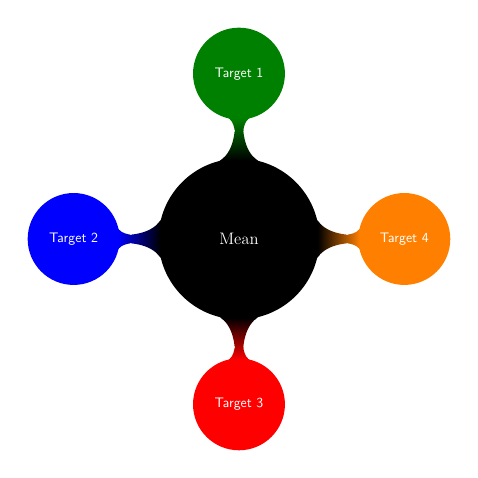
\begin{tikzpicture}[
        level 1 concept/.append style={font=\sf, level distance = 21mm},
        level 2 concept/.append style={font=\sf, level distance = 21mm},
        every node/.append style={scale=0.5}]
        
        \path[mindmap, concept color=black,text=white]
        
        node[concept] {Mean}
        child[grow = 90, concept color=green!50!black] { node[concept] {Target 1}}
        child[grow = 180,concept color=blue] { node[concept] {Target 2}}
        child[grow = 270,concept color=red] { node[concept] {Target 3} }
        child[grow = 360,concept color=orange] { node[concept] {Target 4} };   
    \end{tikzpicture}
    
\end{minipage}

\begin{itemize}
    \item Approach: Bias parameter vectors towards their mean vector:
    \begin{equation*}
            \label{eq:meanreg}
            \min_\Theta \|Y - \Phi \Theta \|^2_F + \lambda \sum\nolimits_{m=1}^l \|\thetab_m - \frac{1}{l} \sum\nolimits_{m'=1}^l \thetab_{m'} \|^2 \, ,
    \end{equation*}
    
%    \item The assumption that all target models are similar is too strict.
\end{itemize}
{\tiny Evgeniou and Pontil, Regularized multi--task learning, KDD 2004}
\end{frame}


\begin{frame}{Stacking (Stacked generalization)}
	
	\begin{itemize}
	
		\item Originally introduced as a general ensemble learning or blending technique.
		
		\item Level 1 learners: apply a series of ML methods on the same dataset (or, one ML method on bootstrap samples of the dataset)
		\item Level 2 learner: apply an ML method to a new dataset consisting of the predictions obtaining at Level 1 
	\end{itemize}
	
	\begin{center}
		\def\layersep{1.25cm}
		\begin{tikzpicture}[shorten >=1pt,->,draw=black!50, node distance=\layersep]
			\tikzstyle{every pin edge}=[<-,shorten <=1pt]
			\tikzstyle{neuron}=[circle,fill=black!25,minimum size=17pt,inner sep=0pt]
			\tikzstyle{input neuron}=[neuron, fill=green!50];
			\tikzstyle{output neuron}=[neuron, fill=red!50];
			\tikzstyle{hidden neuron}=[neuron, fill=blue!50];
			\tikzstyle{annot} = [text width=4em, text centered]
			
			% Draw the input layer nodes
			\foreach \name / \y in {1,...,4}
			% This is the same as writing \foreach \name / \y in {1/1,2/2,3/3,4/4}
			\node[input neuron] (I-\name) at (\y, 0) {$f_\y$};
			
			% Draw the hidden layer nodes
			\foreach \name / \y in {1}
			% \path%[yshift=0.5cm]
			\node[hidden neuron] (H-\name) at (2.5, \layersep) {$h_\y$};
			
			
			% % Draw the output layer node
			\node[output neuron] (I) at (2.5, -\layersep) {$\xv$};
			%%
			%%    % Connect every node in the input layer with every node in the
			%%    % hidden layer.
			\foreach \source in {1,...,4}
			\foreach \dest in {1}
			\path (I-\source) edge (H-\dest);
			%%
			%    % Connect every node in the hidden layer with the output layer
			\foreach \source in {1,...,4}
			\path (I) edge (I-\source);
			%
			% Annotate the layers
			\node[annot,left of=H-1, node distance=3cm] (hl) {Level 2}; 
			\node[annot,below of=hl, node distance=\layersep] {Level 1};
			%%    \node[annot,right of=hl] {Output layer};
		\end{tikzpicture}
	\end{center}
	{\tiny Wolpert, Stacked generalization. Neural Networks 1992.}
\end{frame}

\begin{frame}{Stacking applied to MTP }
	\begin{minipage}{0.5\textwidth}
        \begin{itemize}
            \item Level 1: learn $f(\xv)_1,\ldots,f(\xv)_l$ independently.
        
            \item Level 2: learn a model for each target independently, using the predictions of the first step
            $\leadsto$ $f(\xv) = g(f(\xv)_1,\ldots,f(\xv)_l)$ \\
            Or: $f(\xv) = g(f(\xv)_1,\ldots,f(\xv)_l,\xv)$  \\ 
        \end{itemize}
	\end{minipage}
    \hfill
    \begin{minipage}{0.45\textwidth}
        \def\layersep{2cm}
        \begin{tikzpicture}[shorten >=1pt,->,draw=black!50, node distance=\layersep]
            \tikzstyle{every pin edge}=[<-,shorten <=1pt]
            \tikzstyle{neuron}=[circle,fill=black!25,minimum size=17pt,inner sep=0pt]
            \tikzstyle{input neuron}=[neuron, fill=green!50];
            \tikzstyle{output neuron}=[neuron, fill=red!50];
            \tikzstyle{hidden neuron}=[neuron, fill=blue!50];
            \tikzstyle{annot} = [text width=4em, text centered]
            
            % Draw the input layer nodes
            \foreach \name / \y in {1,...,4}
            % This is the same as writing \foreach \name / \y in {1/1,2/2,3/3,4/4}
            \node[input neuron] (I-\name) at (\y, 0) {$f_\y$};
            
            % Draw the hidden layer nodes
            \foreach \name / \y in {1,...,4}
            % \path%[yshift=0.5cm]
            \node[hidden neuron] (H-\name) at (\y, \layersep) {$g_\y$};
            
            
            % % Draw the output layer node
            \node[output neuron] (I) at (2.5, -\layersep) {$\xv$};
            %%
            %%    % Connect every node in the input layer with every node in the
            %%    % hidden layer.
            \foreach \source in {1,...,4}
            \foreach \dest in {1,...,4}
            \path (I-\source) edge (H-\dest);
            %%
            %    % Connect every node in the hidden layer with the output layer
            \foreach \source in {1,...,4}
            \path (I) edge (I-\source);
            %
            % Annotate the layers
            \node[annot,left of=H-1, node distance=1cm] (hl) {Level 2}; 
            \node[annot,left of=I-1, node distance=1cm] {Level 1};
            %%    \node[annot,right of=hl] {Output layer};
        \end{tikzpicture}    
    \end{minipage}	

	\begin{itemize}
		\item Advantages: easy to implement and general. 
        
		\item Has been shown to avoid overfitting in multivariate regression.
        
		\item If level 2 learner uses regularization $\leadsto$ models are forced to learn similar parameters for different targets.  
	\end{itemize}

	{\tiny Cheng and H\"ullermeier, Combining Instance-based learning and Logistic Regression for Multi-Label classification, Machine Learning, 2009.}
	
\end{frame}

\begin{frame}{Stacking vs Binary Relevance: Example}

   \begin{itemize}
   
       \item Compare F1-Score of random forest with stacking vs random forest with binary relevance on different multilabel datasets:
       
       \begin{center}
       \resizebox{10cm}{!}{
         \begin{tabular}{lrrrrrrrrrr}
           \toprule
           & birds & emotions & enron & genbase & image & langLog & reuters & scene & slashdot & yeast\\
           \midrule
           BR(rf) F1-Score & 0.637 & 0.620 & 0.578 & 0.989 & 0.431 & 0.319 & 0.671 & 0.616 & 0.441 & 0.615\\
           STA(rf) F1-Score & 0.646 & 0.634 & 0.583 & 0.986 & 0.446 & 0.317 & 0.685 & 0.633 & 0.453 & 0.624\\
           \bottomrule
         \end{tabular}
         }
       \end{center}
       
       \item F1-Score is decomposed over targets.

       \item NB: Stacking slightly outperforms binary relevance on average.

       \item For more details, please refer to \href{https://journal.r-project.org/archive/2017/RJ-2017-012/RJ-2017-012.pdf}{\beamergotobutton{Probst et al., 2017 }}.
   \end{itemize}

\end{frame}

\begin{frame}{Enforcing similarity in Deep Learning}
	\begin{center}
		Commonly-used architecture: weight sharing in the final layer with $m$ nodes, i.e., weight sharing among the targets \\
		\includegraphics[scale=0.4]{figure/weightsharing}
	\end{center}

    {\tiny Caruana, Multitask learning: A knowledge-based source of inductive bias. Machine	Learning 1997.}
\end{frame}

\endlecture
\end{document}
